\section{Auswertung}
\subsection{Bestimmung der Schallgeschwindigkeit}

Die Messwerte zur Bestimmung der Schallgeschwindigkeit in Acryl sind in Tabelle
\ref{tab:tabe1} abzulesen.
\begin{table}[H]
  \centering
  \caption{Messwerte der Wärmepumpe}
  \label{tab:tabe1}
    \begin{tabular}{S S S S S S}
    \toprule
    $ t  \: / \si{\second} $ & $ p_a \: / \si{\bar} $ & $ p_b \: / \si{\bar} $ &
    $ T_1 \: / \si{\kelvin} $ & $ T_2 \: / \si{\kelvin} $ & $ P \: / \: \si{\watt} $\\
    \midrule
    0 & 5.0 & 5.0 & 293.65 & 293.65 & 0 \\
    60 & 4.7 & 6.0 & 294.15 & 293.55 & 115 \\
    120 & 4.4 & 6.4 & 295.15 & 293.15 & 118 \\
    180 & 4.5 & 6.9 & 296.35 & 291.95 & 122 \\
    240 & 4.6 & 7.0 & 297.55 & 290.95 & 125 \\
    300 & 4.6 & 7.0 & 298.85 & 289.95 & 125 \\
    360 & 4.5 & 7.2 & 300.05 & 289.15 & 123 \\
    420 & 4.4 & 7.4 & 301.15 & 288.45 & 123 \\
    480 & 4.3 & 7.8 & 302.35 & 287.65 & 122 \\
    540 & 4.2 & 8.0 & 303.55 & 286.95 & 122 \\
    600 & 4.2 & 8.1 & 304.65 & 286.25 & 121 \\
    660 & 4.1 & 8.3 & 305.75 & 285.55 & 121 \\
    720 & 4.0 & 8.5 & 306.75 & 284.95 & 121 \\
    780 & 4.0 & 8.8 & 307.75 & 284.35 & 121 \\
    840 & 3.9 & 9.0 & 308.75 & 283.75 & 121 \\
    900 & 3.8 & 9.1 & 309.65 & 283.15 & 121 \\
    960 & 3.8 & 9.2 & 310.55 & 282.55 & 122 \\
    1020 & 3.8 & 9.5 & 311.45 & 282.05 & 122 \\
    1080 & 3.7 & 9.8 & 312.25 & 281.55 & 122 \\
    1140 & 3.7 & 10.0 & 313.05 & 281.15 & 122 \\
    1200 & 3.7 & 10.0 & 313.9 & 280.65 & 122 \\
    1260 & 3.6 & 10.2 & 314.65 & 280.25 & 123 \\
    1320 & 3.6 & 10.3 & 315.35 & 279.85 & 123 \\
    1380 & 3.6 & 10.6 & 316.15 & 279.45 & 124 \\
    1440 & 3.6 & 10.8 & 316.85 & 279.15 & 124 \\
    1500 & 3.6 & 11.0 & 317.55 & 278.75 & 124 \\
    1560 & 3.6 & 11.1 & 318.25 & 278.55 & 124 \\
    1620 & 3.6 & 11.2 & 318.95 & 278.25 & 125 \\
    1680 & 3.5 & 11.4 & 319.55 & 277.95 & 125 \\
    1740 & 3.5 & 11.5 & 320.15 & 277.65 & 125 \\
    1800 & 3.5 & 11.7 & 320.75 & 277.45 & 125 \\
    1860 & 3.5 & 11.9 & 321.35 & 277.25 & 125 \\
    1920 & 3.5 & 12.0 & 321.95 & 277.05 & 125 \\
    1980 & 3.5 & 12.1 & 322.45 & 276.95 & 125 \\








      \bottomrule
    \end{tabular}
\end{table}

Hieraus ergibt sich durch die Gleichung
\begin{equation}
  c = 2\frac{\text{l}}{\increment t}
\end{equation}
eine Schallgeschwindigkeit von $ \SI{2707.42}{\meter\per\second}$.
Die zugehörige Graphik ist in Abbildung \ref{fig:bums} zu sehen.
\begin{figure}[H]
  \centering
  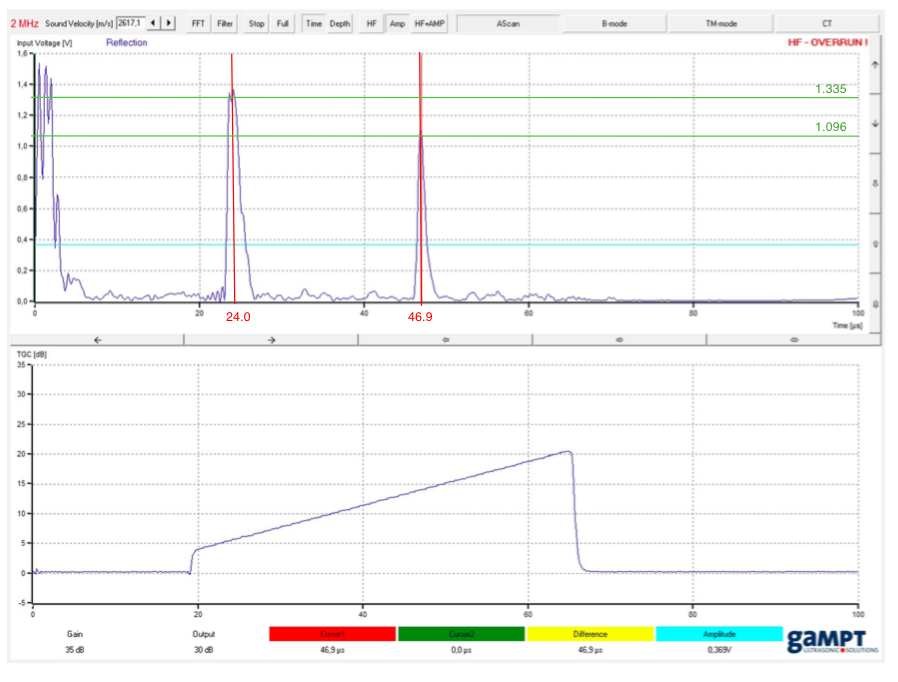
\includegraphics[height=13cm]{Bums.png}
  \caption{Graphik zur Bestimmung der Schallgeschwindigkeit.}
  \label{fig:bums}
\end{figure}

\subsection{Bestimmung der Dämpfung mit dem Impuls-Echo-Verfahren}
Die gemessenen Daten zur Bestimmung der Dämpfung befinden sich in Tabelle
\ref{tab:tabe2}.
\begin{table}[H]
  \centering
  \caption{Wertetabelle für $\alpha$ und $C_V$.}
  \label{tab:tab2}
    \begin{tabular}{S S S S S}
    \toprule
    $ T\: \text{in}\: \si{\K} $ & $ {\alpha \cdot 10^{-6} \: \text{in}\: \si {\per\K}} $ &
    $ C_V \: \text{in}\: \si{\J\per\K\mol} $\\
    \midrule %Cv, a *10-6, Cv
    %0 & 1 & 1\\
    88.60\pm0.24 & 9.56\pm0.06 & 14.17\pm8.13  \\ %&3.6 & 318.97\pm0.85\\
    93.81\pm0.24 & 10.10\pm0.06 & 17.58\pm10.03 \\ %& 4.7 & 440.90\pm1.11\\
    99.74\pm0.24 & 10.66\pm0.05 & 15.52\pm8.84 \\ %& 5.1 & 508.68\pm1.21\\
    104.74\pm0.24 & 11.07\pm0.05 & 18.44\pm10.52 \\ %& 4.6 & 481.79\pm1.09\\
    110.94\pm0.24 &  11.54\pm0.05 & 14.86\pm8.45 \\ %& 5.3 & 587.97\pm1.27\\
    115.96\pm0.24 & 11.89\pm0.05 & 18.49\pm10.52 \\ %& 4.6 & 533.41\pm1.10\\
    121.47\pm0.24 &  12.22\pm0.05 & 16.83\pm9.57 \\ %& 4.9 & 595.21\pm1.17\\
    126.99\pm0.24 & 12.53\pm0.04 & 16.79\pm9.54 \\ %& 4.9 & 622.29\pm1.18\\
    131.58\pm0.24 & 12.77\pm0.04 & 20.42\pm11.62 \\ %& 4.2 & 552.62\pm1.01\\
    136.65\pm0.24 & 13.02\pm0.04 & 18.40\pm10.47 \\ %& 4.6 & 628.57\pm1.11\\
    141.49\pm0.24 & 13.24\pm0.04 & 19.28\pm10.97 \\ %& 4.4 & 622.54\pm1.07\\
    146.34\pm0.24 & 13.44\pm0.04 & 19.24\pm10.95 \\ %& 4.4 & 643.88\pm1.07\\
    150.95\pm0.24 & 13.62\pm0.04 & 20.22\pm11.52 \\ %& 4.3 & 649.11\pm1.05\\
    155.34\pm0.24 & 13.79\pm0.04 & 21.31\pm12.14 \\ %& 4.1 & 636.88\pm0.98\\
    159.97\pm0.24 & 13.95\pm0.04 & 20.12\pm11.47 \\ %& 4.3 & 687.89\pm1.05\\
    164.62\pm0.24 & 14.10\pm0.04 & 20.18\pm11.51 \\ %& 4.3 & 707.87\pm1.06\\
    168.79\pm0.25 & 14.23\pm0.04 & 22.54\pm12.86 \\ %& 3.9 & 658.27\pm0.95\\
    173.45\pm0.25 &  14.37\pm0.04 & 20.08\pm11.46 \\ %& 4.3 & 745.84\pm1.06\\
    178.13\pm0.25 &  14.50\pm0.04 & 20.04\pm11.44 \\ %& 4.3 & 765.94\pm1.06\\
    182.56\pm0.25 &  14.62\pm0.04 & 21.11\pm12.06\\
    192.70\pm0.25 &  14.87\pm0.04 & 18.41\pm10.47\\
    200.15\pm0.25 &  15.04\pm0.04 & 25.19\pm14.28\\
    208.87\pm0.25 &  15.23\pm0.04 & 21.43\pm12.18\\
    217.12\pm0.25 &  15.38\pm0.04 & 22.65\pm12.88\\
    225.15\pm0.25 &  15.53\pm0.03 & 23.27\pm13.24\\
    232.70\pm0.25 &  15.70\pm0.03 & 24.75\pm14.08\\
    240.53\pm0.25 &  15.74\pm0.03 & 23.84\pm13.58\\
    248.39\pm0.25 &  15.89\pm0.03 & 23.74\pm13.53& \\
    256.01\pm0.25 &  15.97\pm0.03 & 24.46\pm13.94 \\
    263.41\pm0.26 &  16.01\pm0.03 & 25.22\pm14.38 \\
    271.08\pm0.26 &  16.18\pm0.03 & 24.26\pm13.86 \\
    278.52\pm0.26 &  16.27\pm0.03 & 25.03\pm14.29&\\
    285.98\pm0.26 &  16.35\pm0.03 & 24.92\pm14.25 \\
    293.21\pm0.26 &  16.42\pm0.03 & 25.74\pm14.72 \\
    300.98\pm0.26 &  16.50\pm0.03 & 23.87\pm13.68 \\
    308.51\pm0.26 &  16.57\pm0.03 & 24.63\pm14.12\\



      \bottomrule
    \end{tabular}
\end{table}

Durch Umstellung der Gleichung \ref{eqn:intensität} ergibt sich die Gleichung
\begin{equation}
  - \text{ln}(\frac{\text{I}}{\text{I}_0})= x \cdot \alpha \: ,
\end{equation}
sodass sich die Dämpfungskonstante durch eine lineare Ausgleichsrechnung der Form
\begin{equation}
  y = a\cdot x +b
  \label{eqn:linear}
\end{equation}
mit den Wertepaaren aus $\text{ln}(\frac{\text{I}}{\text{I}_0})$ und $2 \cdot$l
ergibt. Die Werte sind zusammen mit der Ausgleichsgrade in Abbildung \ref{fig:plot1}
dargestellt.
\begin{figure}[H]
  \centering
  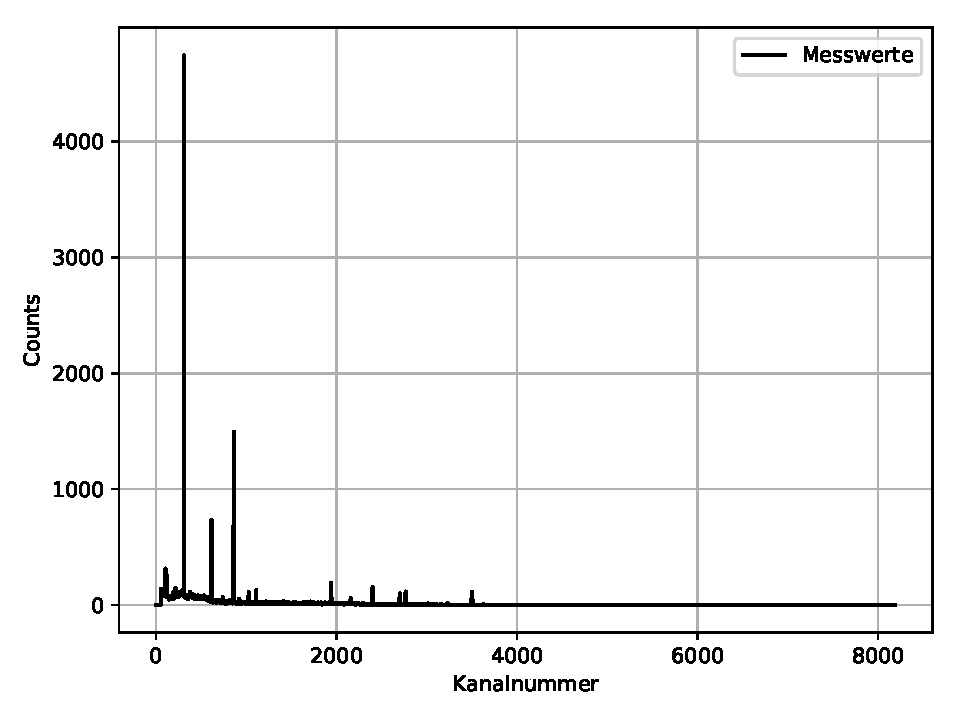
\includegraphics[height=6cm]{plot1.pdf}
  \caption{Wertepaare und Ausgleichsgrade}
  \label{fig:plot1}
\end{figure}
Hieraus ergeben sich die Parameter:
\begin{align*}
  a &= 0,020 \pm 0,002 \: \frac{1}{\text{mm}} \\
  b &= 1,4 \pm 0,3
\end{align*}
Die zu bestimmende Dämpfungskonstante ergibt sich somit insgesamt zu
\begin{align*}
  \alpha = 0,020 \pm 0,002 \: \frac{1}{\text{mm}} \: .
\end{align*}

\subsection{Schallgeschwindigkeitsbestimmung mit dem Impuls-Echo-Verfahren}
Die gemessenen Wertepaare sind, zusammen mit den daraus errechneten
Schallgeschwindigkeiten, in Tabelle \ref{tab:tabe3} aufgeführt.
\begin{table}
  \centering
  \caption{Messwerte für den ersten Doppelspalt.}
   \begin{tabular}{S S| S S | S S}
    \toprule
    $x/\; \si{\mm}$& $A/\;\si{\nA}$ &
    $x/\; \si{\mm}$& $A/\;\si{\nA}$ &
    $x/\; \si{\mm}$& $A/\;\si{\nA}$ \\
    \midrule

    15.0& 4.6& 23.0& 25.0& 29.5& 6.0\\
    15.5& 4.2& 23.5& 30.0& 30.0& 5.3\\
    16.0& 4.0& 24.0& 35.0& 30.5& 4.9\\
    16.5& 4.0& 24.25& 36.0& 31.0& 4.7\\
    17.0& 4.4& 24.5& 37.0& 31.5& 4.4\\
    17.5& 5.5& 24.75& 38.0& 32.0& 4.2\\
    18.0& 6.6& 25.00& 37.0& 32.5& 3.8\\
    18.5& 7.7& 25.25& 36.0& 33.0& 3.6\\
    19.0& 8.2& 25.5& 36.0& 33.5& 3.2\\
    19.5& 8.4& 26.0& 33.0& 34.0& 3.2\\
    20.0& 8.4& 26.5& 28.5& 34.5& 3.2\\
    20.25& 8.4& 27.0& 23.0& 35.0& 3.3\\
    20.5& 8,7& 27.5& 18.0& 35.5& 3.4\\
    21.0& 9.8& 28.0& 13.5& 36.0& 3.5\\
    21.5& 12.0& 28.5& 10.0\\
    22.0& 15.0& 29.0& 7.8\\
    22.5& 20.0& 29.25& 6.7\\


   \bottomrule
  \end{tabular}
  \label{tab:tabelle3}
\end{table}

Aufgrund der Anpassungsschicht weisen die Schallgeschwindigkeiten einen systematischen
Fehler auf, %da sich die Durchlaufgeschwindigkeit aus dem Durchlaufen der Schicht und
%aus dem Durchlaufen des Zylinders zusammensetzt, gemäß der Formel
%\begin{equation}
%  t_{\text{gemessen}} = \frac{2\cdot l}{c} + \frac{2 \cdot l_a}{c_w} \: ,
%\end{equation}
%wobei $l_a$ die Dicke der Anpassungsschicht angibt und $c_w = \SI{1480}{\meter\per\second}$
%die Schallgeschwindigkeit in destilliertem Wasser.
%Es lässt sich also ein
%\begin{equation}
%  \increment t = \frac{t_{\text{gemessen}}}{2} - \frac{l}{c}
%\end{equation}
%bestimmen, welches die Laufzeit in der Anpassungsschicht angibt, wodurch sich die
%Dicke der Anpassungsschicht zu
%\begin{equation}
%  l_a = \increment t  \cdot c_w
%\end{equation}
%ergibt. Die somit berechneten Werte für die Anpassungsschicht sind in Tabelle \ref{tab:tabe6}
%aufgeführt.
%\begin{table}[H]
  \centering
  \caption{Werte der Anpassungsschicht}
  \label{tab:tabe6}
    \begin{tabular}{S S S }
    \toprule
    $ \text{Zylinder} $ & $ \increment t [\mu\text{s}] $ &
    $ l_a \text{[mm]}$\\
    \midrule
    1 & 0.54 & 0.81 \\
    2 & 0.40 & 0.59 \\
    3 & 0.76 & 1.12 \\
    \text{1+2} & 0.49 & 0.73 \\
    4 & 0.70 & 1.03 \\
    \text{1+3} & 0.90 & 1.33 \\
    5 & 1.25 & 1.85 \\
    \text{1+4} & 0.69 & 1.02 \\
    6 & 0.44 & 0.66 \\

          \bottomrule
    \end{tabular}
  \end{table}

%Durch die Gleichung
%\begin{equation}
%  \bar{x} = \frac{1}{N} \sum_{i=1}^{N} x_i \: \:
%  \label{eqn:mit}
%\end{equation}
%\noindent lässt sich der Mittelwert bilden, wobei der dazugehörige Fehler sich durch
%\begin{equation}
%  \increment \bar{x} = \frac{1}{\sqrt{N}} \sqrt{ \frac{1}{N-1} \sum_{i=1}^N
%  (x_i - \bar{x})^2}
%  \label{eqn:mitf}
%\end{equation}
%ergibt. Somit ergibt sich insgesamt:
%\begin{align*}
%  \increment t &= \SI{0.68(9)}{\micro\second} \\
%  l_a &= \SI{1.01(13)}{\milli\meter}
%\end{align*}
welcher sich durch eine lineare Ausgleichsrechnung durch Gleichung \ref{eqn:linear}
bestimmen lässt, wobei für die x-Werte die Länge der Zylinder verwendet werden und
für die y-Werte die Durchlaufzeit. Die Wertepaare sind zusammen mit der
Ausgleichsgeraden in Abbildung \ref{fig:plot2} dargestellt.
\begin{figure}[H]
  \centering
  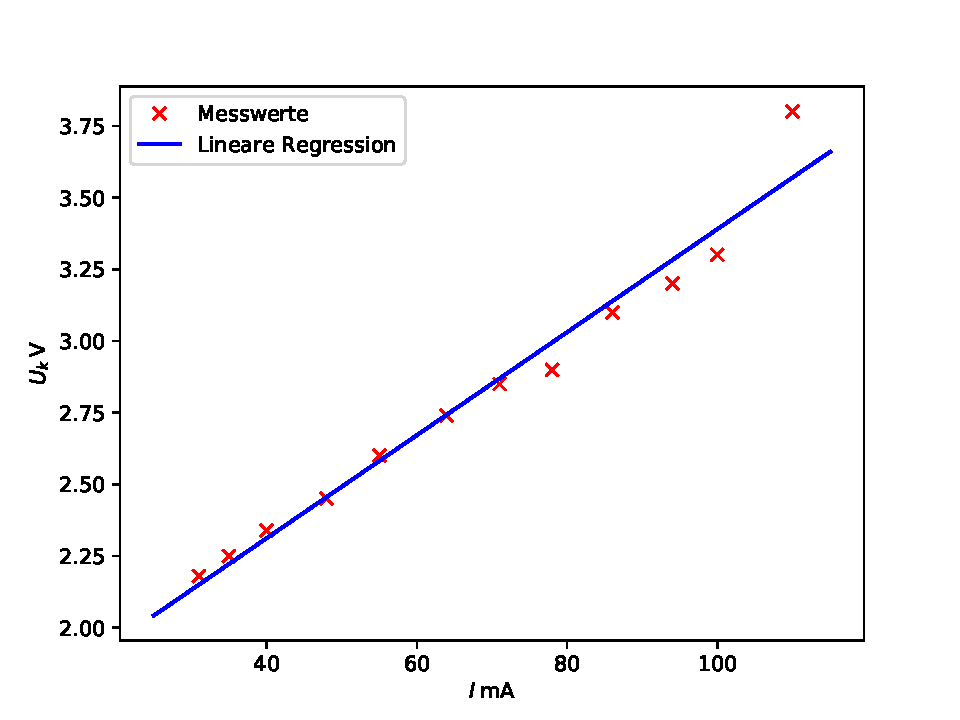
\includegraphics[height=6cm]{plot2.pdf}
  \caption{Wertepaare und Ausgleichsgrade}
  \label{fig:plot2}
\end{figure}
Hieraus ergeben sich die Parameter:
\begin{align*}
  a &= 0,370 \pm 0,004 \: \frac{\mu s}{\text{mm}} \\
  b &= 0,85 \pm 0,6 \: \mu s
\end{align*}
Der y-Achsenabschnitt gibt hierbei die Zeit zum zweimaligen Durchlaufen der Anpassungsschicht
an. Durch Division mit 2 und Multiplikation mit der Schallgeschwindigkeit $c_w = \SI{1480}{\meter\per\second}$
in destilliertem Wasser lässt sich somit die Dicke der Anpassungsschicht bestimmen,
wodurch sich insgesamt die Werte
\begin{align*}
  t_a &= \SI{0.43(3)}{\micro\second} \\
  l_a &= \SI{0.64(4)}{\milli\meter}
\end{align*}
ergeben.


\subsection{Schallgeschwindigkeitsbestimmung mit dem Durchschallungsverfahren}
Die gemessenen Werte befinden sich zusammen mit den daraus errechneten Schallgeschwindigkeiten
in Tabelle \ref{tab:tabe4}.
\begin{table}[H]
  \centering
   \begin{tabular}{c c c c}
    \toprule
    Nummer der Oberwelle & $ U_{\text Theorie,Rechteck}\: / \si{\volt} $ &
    $ U_{\text Theorie,Dreick}\: / \si{\volt} $ & $ U_{\text Theorie,Sägezahn}\: / \si{\volt} $ \\
    \midrule
    1 & 1145 & 182 & 573 \\
    2 & 0 & 0 & 286 \\
    3 & 573 & 20 & 191 \\
    4 & 0 & 0 & 143 \\
    5 & 229 & 7 & 115 \\
    6 & 0 & 0 & 96 \\
    7 & 164 & 4 & 82 \\
    8 & 0 & 0 & 72 \\
    9 & 127 & 2 & 64 \\
    10 & 0 & 0 & 57 \\
    \bottomrule
  \end{tabular}
  \caption{Eingestellte Schwingungsamplituden.}
  \label{tab:tabe4}
\end{table}


\subsection{Spektrale Analyse und Cepstrum}
In Abbildung \ref{fig:cep} sind das Spektrum und Cepstrum der Mehrfachreflexionen
dargestellt.
\begin{figure}[H]
  \centering
  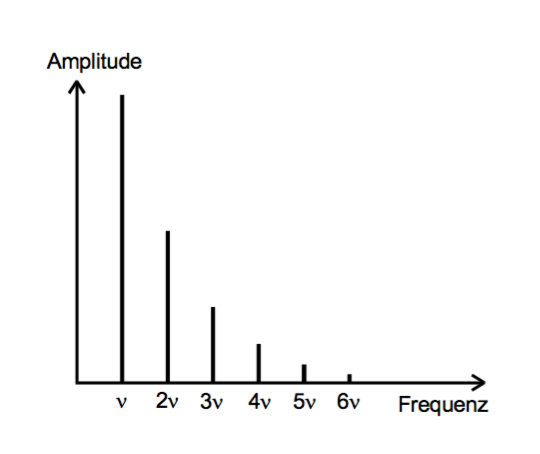
\includegraphics[height=12cm]{Spektrum.pdf}
  \caption{Spektrum und Cepstrum der Mehrfachreflexionen}
  \label{fig:cep}
\end{figure}

\subsection{Biometrische Untersuchung eines Augenmodells}
Die Messung des Augenmodells ist in Abbildung \ref{fig:messauge} dargestellt.
\begin{figure}[H]
  \centering
  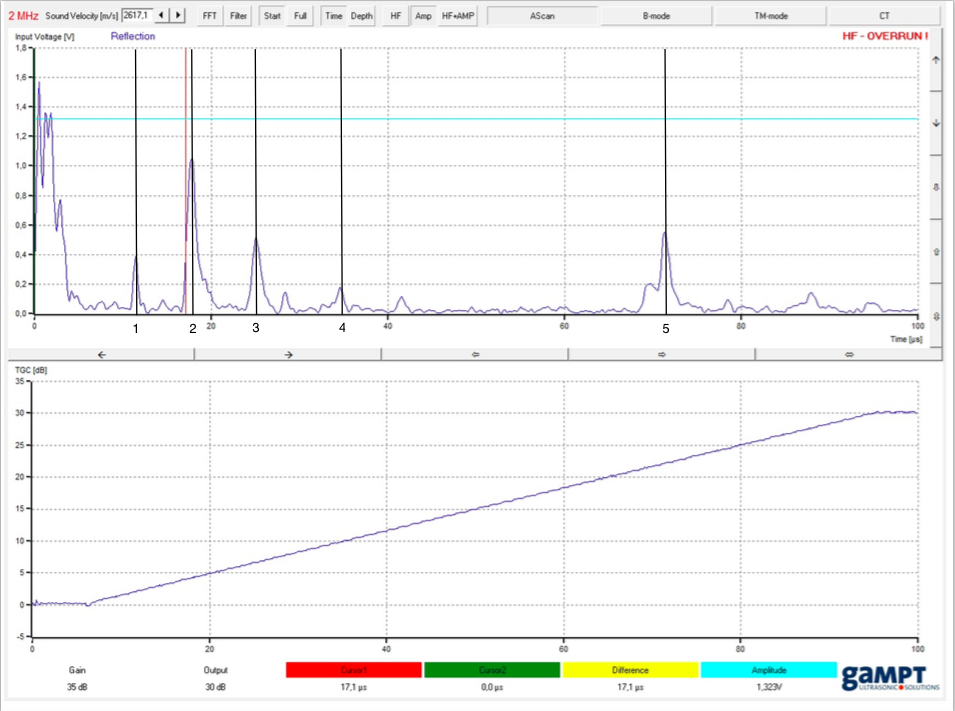
\includegraphics[height=12cm]{Auge2.png}
  \caption{Messung des Auges}
  \label{fig:messauge}
\end{figure}
Die Impulse liegen dabei bei den Zeiten:
\begin{table}[H]
  \centering
  \caption{Bohrung 1 und 2, Vergleich der Sonden mit 1\;MHz und 2\;MHz.}
  \label{tab:tab5}
    \begin{tabular}{c c c c}
    \toprule
    Bohrung & $S_{\text{2\;MHz}}$/\;mm & $S_{\text{ 1\;MHz}}$/\;mm\\
    \midrule
    1 & 1,82 & 2,12\\
    2 & 1,83 & 1,97\\
    \bottomrule
    \end{tabular}
  \end{table}

Der Impuls 1 kommt hierbei durch die Reflexion am Beginn der Linse zustande, sodass
sich dieser Abstand durch die Gleichung
\begin{equation}
  s_1 = \frac{1}{2} \cdot c_{GK} \cdot t_1 \: ,
\end{equation}
ergibt, wobei die Schallgeschwindigkeit $c_{GK}$ in der Glaskörperflüssigkeit $\SI{1410}{\meter\per\second}$
beträgt. Dieser Abstand beträgt somit
\begin{align*}
  s_1 = \SI{8.037}{\milli\meter} \: .
\end{align*}
Der zweite Impuls ist bedingt durch Reflexion am Ende der Linse, sodass sich durch die
Formel
\begin{equation}
  s_2 = \frac{1}{2} \cdot c_L \cdot (t_2-t_1)
\end{equation}
mit der Schallgeschwindigkeit $c_L = \SI{2500}{\meter\per\second}$ die Breite der
Linse bestimmen lässt. Diese beträgt somit
\begin{align*}
  s_2 = \SI{7.875}{\milli\meter} \: .
\end{align*}
Die nächsten beiden Impulse kommen durch Mehrfachreflexionen zustanden, sodass diese
keine weiteren Informationen über das Augenmodell liefern. Der fünfte Impuls entsteht
durch Reflexion an der Rückwand des Auges, sodass sich der Abstand vom Ende der
Linse bis zum Ende des Auges durch
\begin{equation}
  s_3 = \frac{1}{2} \cdot c_{GK} \cdot (t_5-t_2)
\end{equation}
zu
\begin{align*}
  s_3 = \SI{37.859}{\milli\meter}
\end{align*}
ergibt.
Der Gesamtdurchmesser des Auges beträgt somit
\begin{align*}
  D = s_1 + s_2 + s_3 = \SI{53.771}{\milli\meter} \: .
\end{align*}
